\documentclass[conference]{IEEEtran}
\IEEEoverridecommandlockouts
% The preceding line is only needed to identify funding in the first footnote. If that is unneeded, please comment it out.
\usepackage{cite}
\usepackage{amsmath,amssymb,amsfonts}
\usepackage{algorithmic}
\usepackage{graphicx}
\usepackage{textcomp}
\usepackage{xcolor}
\def\BibTeX{{\rm B\kern-.05em{\sc i\kern-.025em b}\kern-.08em
    T\kern-.1667em\lower.7ex\hbox{E}\kern-.125emX}}
\begin{document}

\title{Deep Reinforcement Learning-Based Physiological Control for Ventricular Assist Devices}

\author{
\IEEEauthorblockN{Liangzhu Chen}
\IEEEauthorblockA{
\textit{University of Science and Technology of China} \\
Hefei, China \\
chenlz@mail.ustc.edu.cn
}
}

\maketitle

\begin{abstract}
Ventricular assist devices are important therapies for end-stage heart failure, but constant-speed operation cannot adequately match changing physiological demand and may increase the risk of suction, regurgitation, and hemolysis. This paper presents a deep reinforcement learning-based physiological control method for ventricular assist devices. The proposed controller adopts an actor-critic framework with a hybrid CNN-Transformer representation module, where the CNN extracts local waveform morphology and the Transformer captures long-range temporal dependencies across cardiac cycles. A multi-objective reward function is designed to jointly encourage perfusion matching, hemodynamic stability, smooth pump-speed regulation, and safety-related constraint satisfaction. The method is evaluated through a staged pipeline including mock circulatory loop scenarios, offline representation pretraining, online reinforcement learning, comparative transition tests, robustness analysis, and architectural ablation. The results indicate that the proposed framework improves physiological adaptability, disturbance tolerance, and safety-aware pump-speed regulation compared with conventional and weaker learning-based baselines.
\end{abstract}

\begin{IEEEkeywords}
ventricular assist device, physiological control, deep reinforcement learning, actor-critic, CNN-Transformer, hemodynamic regulation
\end{IEEEkeywords}

\section{Introduction}
Heart failure remains a major global health challenge, and the growing aging population continues to increase the number of patients with end-stage cardiac dysfunction \cite{b1}. Ventricular assist devices (VADs) have become an important therapy for these patients because they can provide mechanical circulatory support when the native heart is unable to maintain sufficient perfusion \cite{b3}. However, most currently deployed VADs still operate under constant pump speed settings. Although this strategy is simple and reliable, it cannot dynamically match the patient's changing physiological demand during transitions such as rest, exercise, and recovery \cite{b2,b3}. As a result, constant-speed control may lead to insufficient physiological perfusion and may increase the risk of adverse events including suction, regurgitation, and hemolysis.

To improve the physiological adaptability of VADs, many studies have explored closed-loop control strategies. Traditional methods, including pressure-based feedback control, fuzzy control, and Starling-like control, can improve performance under specific operating conditions \cite{b4,b5,b6,b7}. Nevertheless, these approaches usually depend on simplified cardiovascular models, handcrafted rules, or manually tuned parameters. Because the cardiovascular system is highly nonlinear, time-varying, and patient-specific, model-based or rule-based controllers often struggle to maintain robust performance under complex hemodynamic disturbances. In addition, control objectives in VAD applications are inherently multi-objective, requiring the controller to simultaneously satisfy perfusion demand, maintain hemodynamic stability, and avoid complications. These requirements make conventional control design increasingly difficult.

Recent advances in artificial intelligence have created new opportunities for physiological control of biomedical devices \cite{b8,b9}. In particular, deep reinforcement learning (DRL) is attractive for VAD control because it can learn control policies directly from data without requiring an accurate explicit model of the cardiovascular system. Existing DRL-based studies have demonstrated the potential of reinforcement learning for pump speed regulation \cite{b2,b14,b16}, but important limitations remain. Some methods rely on multilayer perceptrons or recurrent architectures with limited ability to jointly capture local waveform patterns and long-range temporal dependencies in physiological signals. Other methods focus on a narrow set of reward objectives and therefore do not fully reflect the safety-critical requirements of VAD operation. Consequently, there is still a need for a control framework that combines stronger physiological state representation with a more comprehensive reward design.

To address these issues, this paper proposes a deep reinforcement learning-based physiological control method for ventricular assist devices. The proposed approach adopts an actor-critic framework with a hybrid CNN-Transformer architecture, where the CNN module extracts local features from pressure and flow signals and the Transformer module models long-range temporal dependencies across cardiac cycles. A multi-objective reward function is further designed to encourage adequate physiological perfusion while reducing the risks of suction, regurgitation, and hemolysis. The main contributions are threefold: 1) a CNN-Transformer actor-critic control architecture for hemodynamic state perception from sequential physiological signals; 2) a reward design that integrates perfusion regulation, control smoothness, and complication avoidance; and 3) a staged evaluation pipeline covering transition tracking, disturbance robustness, safety behavior, and architectural ablation.

\section{Related Work}
Existing VAD control strategies have evolved from constant-speed operation to more advanced physiological control schemes \cite{b3}. Conventional closed-loop methods, including pressure-based feedback control, proportional-integral regulation, fuzzy control, and Starling-like control, have shown the ability to improve pump response under specific operating conditions \cite{b4,b5,b6,b7}. These methods are attractive because of their conceptual simplicity and clear control objectives. However, they typically depend on simplified cardiovascular models, manually selected control indicators, or extensive parameter tuning. As a result, their performance may degrade when confronted with the highly nonlinear, time-varying, and patient-specific nature of cardiovascular dynamics. In addition, traditional approaches often optimize a limited set of variables and therefore face difficulties when multiple safety and perfusion objectives must be satisfied simultaneously.

With the development of artificial intelligence, learning-based methods have been introduced to improve state perception and decision making for VAD regulation. Some studies have used recurrent neural networks to classify abnormal and normal physiological states, which helps enhance physiological signal interpretation but is still closer to state recognition than to full closed-loop control \cite{b8}. Other works have incorporated neural networks into existing control architectures to compensate for uncertainties or estimate hidden hemodynamic variables \cite{b10}. Convolutional neural networks have also been explored for sensorless estimation tasks, such as preload estimation from pump flow waveforms, demonstrating the potential of deep models to extract informative features from physiological signals \cite{b12}. Nevertheless, many of these approaches focus on diagnosis, estimation, or auxiliary modeling rather than directly learning an adaptive physiological control policy.

Deep reinforcement learning has further advanced the development of intelligent VAD controllers by offering a data-driven framework for continuous decision making. Recent studies based on PPO, DDPG, and TD3 have shown that reinforcement learning can regulate pump speed according to changing physiological conditions and can improve the adaptability of VAD operation \cite{b2,b14,b16}. Despite this progress, important limitations remain. In several existing studies, the actor and critic networks are built on multilayer perceptrons or recurrent modules that cannot simultaneously capture local waveform variations and long-range temporal dependencies with sufficient effectiveness \cite{b2,b14}. Moreover, some reward designs emphasize only a narrow subset of performance objectives, such as average flow or selected hemodynamic indicators, and therefore do not fully address the safety-critical requirements of VAD control, including the prevention of suction, regurgitation, and hemolysis.

Motivated by these gaps, this work aims to improve both physiological state representation and control objective design in deep reinforcement learning-based VAD regulation. The proposed method combines a CNN-Transformer architecture with an actor-critic framework to jointly model local signal patterns and long-term temporal information. In addition, a multi-objective reward function is introduced to better integrate physiological perfusion demand with safety constraints. In this sense, the present work extends existing research from general intelligent control toward a more comprehensive physiological control framework for ventricular assist devices.

\section{Methods}
This section presents the proposed deep reinforcement learning-based physiological control framework for ventricular assist devices. The overall method formulates VAD regulation as a continuous control problem and combines an actor-critic learning strategy with a CNN-Transformer state representation model and a multi-objective reward mechanism.
The overall architecture of the proposed framework is shown in Fig.~\ref{fig:cnn_transformer_actor_critic}.

\IfFileExists{figures/cnn-transformer-actor-critic-vad.pdf}{
\begin{figure*}[!t]
\centering
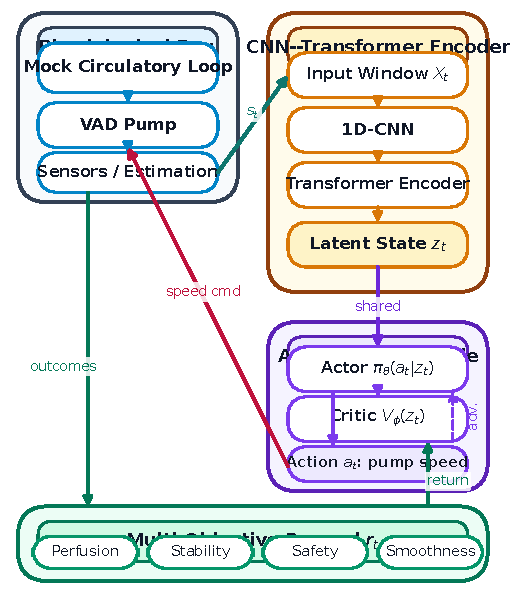
\includegraphics[width=\textwidth]{figures/cnn-transformer-actor-critic-vad.pdf}
\caption{CNN-Transformer actor-critic framework for physiological VAD control. Multichannel physiological waveforms are encoded by a shared CNN-Transformer representation module, where the CNN extracts local waveform morphology and the Transformer captures long-range temporal dependencies across cardiac cycles. The actor outputs adaptive pump speed commands, while the critic evaluates long-term control utility under a multi-objective reward that balances perfusion matching, hemodynamic stability, control smoothness, and safety penalties related to suction, regurgitation, and hemolysis.}
\label{fig:cnn_transformer_actor_critic}
\end{figure*}
}{}

\subsection{Problem Formulation}
The VAD physiological control task is formulated as a sequential decision-making problem. At each control step, the controller receives a state vector composed of measured or estimated physiological signals, such as pressure- and flow-related waveforms and their recent temporal evolution. Based on this information, the controller outputs a continuous pump speed command to regulate the mechanical support provided by the device. The control objective is not only to maintain adequate perfusion under changing physiological demand, but also to preserve hemodynamic stability and reduce the risk of adverse events.

From a reinforcement learning perspective, the physiological state of the cardiovascular system defines the environment state, the pump speed adjustment corresponds to the action, and the immediate control quality is reflected by a reward signal. Because VAD regulation must continuously adapt to nonlinear and patient-specific dynamics, the control policy is required to learn from sequential interactions rather than from a fixed analytical model. This formulation allows the proposed method to address dynamic transitions such as rest-to-exercise changes and other time-varying physiological conditions in a unified framework.

\subsection{Actor-Critic Framework}
The proposed controller is built on an actor-critic reinforcement learning framework, which is well suited for continuous control problems such as pump speed regulation. The actor network maps the current physiological state to a control action, while the critic network evaluates the long-term utility of the policy by estimating the expected return under the current state-action relationship. Through iterative interaction with the environment, the actor is updated to generate more effective physiological control actions, and the critic provides guidance to stabilize policy learning. This design follows the general line of recent DRL-based VAD control studies while extending them with a stronger state representation module \cite{b2,b14,b16}.

Compared with rule-based or purely supervised approaches, the actor-critic framework offers two main advantages in this problem. First, it can directly optimize sequential control performance under long-term physiological objectives instead of relying on manually designed control laws. Second, it can naturally support adaptive decision making in the presence of nonlinear cardiovascular dynamics and operating condition changes. This property is particularly important for VAD control, where the controller must continuously balance support effectiveness and safety under uncertain physiological disturbances.

\subsection{CNN-Transformer Architecture}
To improve physiological state representation, a hybrid CNN-Transformer architecture is adopted in the actor-critic framework. The CNN module is responsible for extracting local morphological features from physiological waveforms. This design is beneficial for identifying short-term signal variations and waveform patterns that may reflect instantaneous hemodynamic changes or early signs of unsafe operating conditions. In the VAD setting, such local information is important because adverse events may first appear as subtle disturbances in pressure or flow signals. The use of convolutional representations is also motivated by prior sensorless estimation studies that showed CNN-based models can effectively capture informative waveform features in VAD applications \cite{b12}.

The Transformer module is introduced to capture long-range temporal dependencies in sequential physiological data. Unlike architectures that mainly focus on local or short-memory representations, the Transformer can model interactions across multiple cardiac cycles and therefore provide a more comprehensive description of evolving hemodynamic states. By combining CNN-based local feature extraction with Transformer-based temporal modeling, the proposed architecture is designed to improve physiological state perception and provide richer representations for both the actor and critic networks. This design is intended to address the representational limitations observed in previous DRL controllers that mainly relied on multilayer perceptrons or recurrent structures \cite{b2,b14,b15,b16}.

\subsection{Reward Design}
A multi-objective reward function is designed to incorporate both physiological regulation and safety constraints into policy learning. The reward encourages the controller to maintain physiologically appropriate perfusion and stable hemodynamic behavior under changing operating conditions. At the same time, it penalizes unsafe or undesirable states associated with suction, regurgitation, and hemolysis, so that the learned policy does not improve one objective at the expense of clinical safety. This formulation extends prior DRL-based VAD reward designs that often emphasized a narrower subset of control objectives \cite{b2,b14,b16}.

The total immediate reward is formulated as a weighted sum of four components:
\begin{equation}
\begin{aligned}
R ={}& w_{\mathrm{perf}} R_{\mathrm{perf}}
+ w_{\mathrm{suction}} R_{\mathrm{suction}} \\
&+ w_{\mathrm{backflow}} R_{\mathrm{backflow}}
+ w_{\mathrm{stab}} R_{\mathrm{stab}},
\end{aligned}
\label{eq:total_reward}
\end{equation}
where $w_{\mathrm{perf}}$, $w_{\mathrm{suction}}$, $w_{\mathrm{backflow}}$, and $w_{\mathrm{stab}}$ are non-negative weights used to balance physiological perfusion, suction prevention, backflow avoidance, and speed smoothness. The perfusion term encourages the mean arterial pressure (MAP) to remain close to a target value:
\begin{equation}
R_{\mathrm{perf}} =
- \exp\left(
\frac{\left|\mathrm{MAP}_{\mathrm{actual}} - \mathrm{MAP}_{\mathrm{target}}\right|}
{\sigma}
\right),
\label{eq:perfusion_reward}
\end{equation}
where $\sigma$ controls the sensitivity to MAP deviation. To reduce the risk of ventricular suction, a penalty is imposed when the minimum left ventricular pressure (LVP) falls below a predefined threshold:
\begin{equation}
R_{\mathrm{suction}} =
\begin{cases}
-C_{\mathrm{penalty}}, & \text{if } \mathrm{LVP}_{\min} < P_{\mathrm{threshold}},\\
0, & \text{otherwise}.
\end{cases}
\label{eq:suction_reward}
\end{equation}
Backflow is penalized when the pump flow $Q_{\mathrm{pump}}$ becomes negative:
\begin{equation}
R_{\mathrm{backflow}} =
-\lambda \max(0, -Q_{\mathrm{pump}}),
\label{eq:backflow_reward}
\end{equation}
where $\lambda$ determines the severity of the backflow penalty. Finally, the control smoothness term discourages abrupt pump speed variations that may increase hemolysis risk:
\begin{equation}
R_{\mathrm{stab}} = -\left|\omega_t - \omega_{t-1}\right|,
\label{eq:stability_reward}
\end{equation}
where $\omega_t$ and $\omega_{t-1}$ denote the current and previous pump speeds, respectively.

This reward design reflects the multi-objective nature of VAD physiological control. In practice, maintaining a single indicator within a desirable range is insufficient, because effective support must simultaneously account for perfusion demand, cardiovascular stability, and complication avoidance. Therefore, the proposed reward mechanism translates clinical and physiological considerations into learning signals that guide the controller toward safer and more adaptive behavior. By embedding these constraints into the reinforcement learning objective, the method aims to achieve a better balance between support performance and operational safety.

\section{Experimental Setup}
The experimental study evaluates the proposed controller under physiologically relevant operating conditions, with emphasis on adaptability, robustness, and safety. The setup combines a controllable simulation or mock circulatory loop environment with staged model development, including offline pretraining and online reinforcement learning.

\subsection{Platform and Physiological Scenarios}
The evaluation platform is designed to reproduce the major hemodynamic characteristics of the cardiovascular system under different physiological conditions. In this study, a controllable simulation environment and a physical mock circulatory loop are considered as complementary testbeds for controller development and validation. The simulation setting provides a flexible environment for large-scale policy interaction during reinforcement learning, whereas the mock circulatory loop offers a more realistic experimental condition with flow inertia, sensor noise, and physical disturbances. This combined setting is intended to narrow the gap between algorithm development and practical implementation.

By adjusting resistance, compliance, preload-related conditions, and other platform parameters, the experiments are configured to represent multiple operating scenarios relevant to VAD support. These scenarios include different levels of heart failure severity, changes in physiological demand associated with rest and activity, and transient operating conditions that require rapid controller adaptation. As a result, the proposed controller is exposed to a broad range of hemodynamic states rather than being validated only in a narrow steady-state regime.

As shown in Fig.~\ref{fig:mcl_platform}, the physical mock circulatory loop platform includes a pulsatile motor, a volume chamber, a compliance chamber, a damping chamber, a flowmeter, and a left ventricular chamber. These components are used to emulate ventricular pumping behavior, vascular compliance, pressure buffering, and flow measurement within a controllable in-vitro environment. The platform therefore provides a practical basis for evaluating whether the proposed controller can maintain appropriate support while responding to realistic disturbances and physiological variations.

\IfFileExists{figures/mcl_platform.png}{
\begin{figure}[t]
\centering
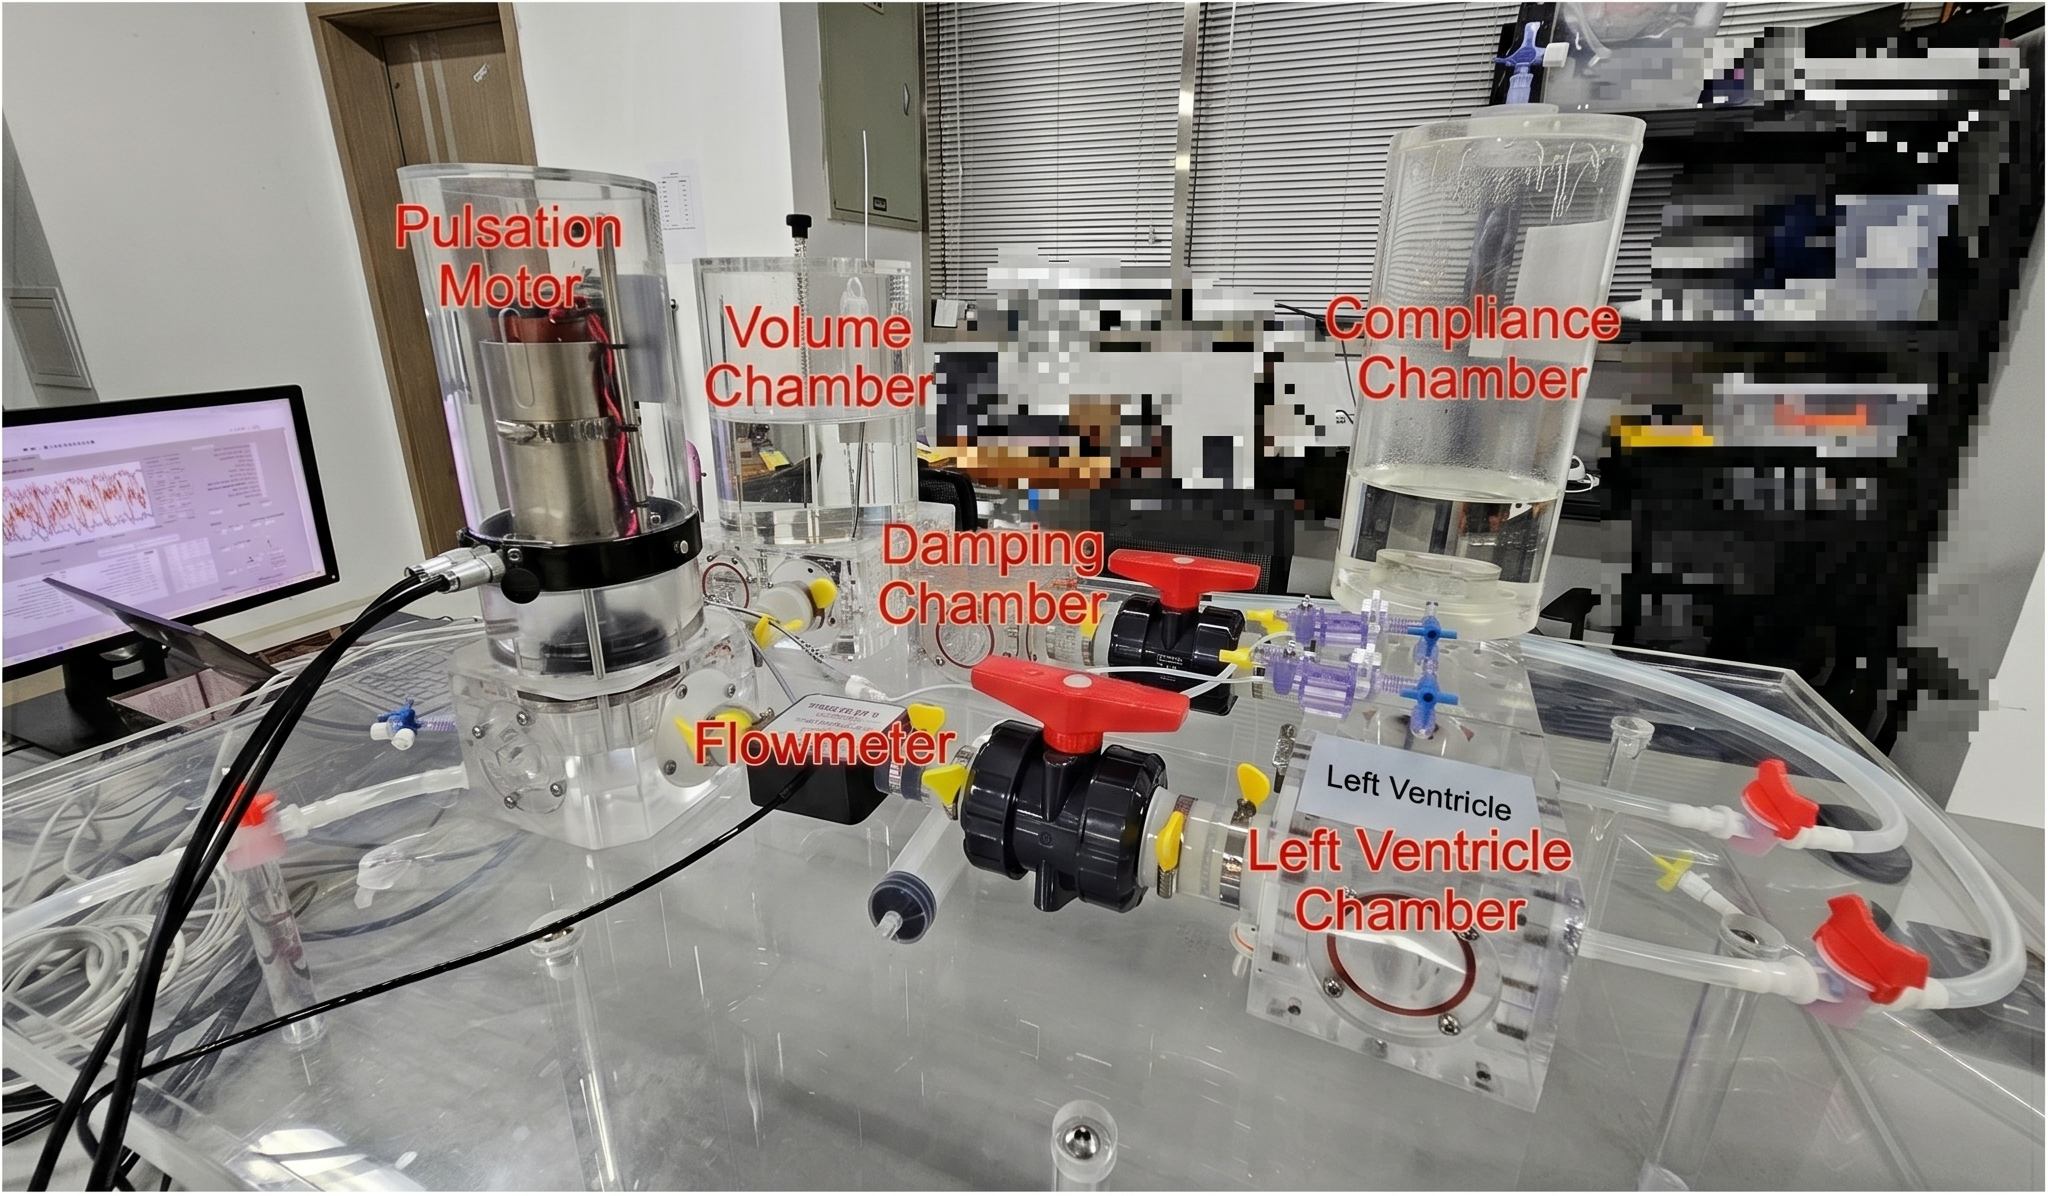
\includegraphics[width=\linewidth]{figures/mcl_platform.png}
\caption{Physical mock circulatory loop platform for ventricular assist device physiological control experiments. The platform includes a pulsatile motor, volume chamber, compliance chamber, damping chamber, flowmeter, and left ventricular chamber to emulate cardiovascular hemodynamic conditions.}
\label{fig:mcl_platform}
\end{figure}
}{}

\subsection{Data Collection and Training Procedure}
The training pipeline follows a staged strategy to improve learning efficiency and stability. In the first stage, representative physiological data are collected under multiple operating conditions by varying platform parameters and recording pressure- and flow-related signals. These data provide broad coverage of different hemodynamic responses and are used to initialize the CNN-Transformer-based representation module before policy optimization. Such offline preparation helps the model capture informative waveform characteristics and reduces the difficulty of learning useful state representations entirely from random exploration.

In the second stage, the controller is further optimized through online reinforcement learning by interacting directly with the simulation environment and, when applicable, the physical test platform. During this process, the actor-critic policy continuously adjusts pump speed according to the observed physiological state, while the reward function guides learning toward adequate perfusion, stable hemodynamics, and reduced risk of unsafe events. This staged procedure is adopted because VAD physiological control involves highly nonlinear dynamics and multi-objective optimization, making purely end-to-end training from scratch more difficult and potentially less stable.

The complete training and evaluation workflow is summarized in Fig.~\ref{fig:training_evaluation_pipeline}. The pipeline connects physiological scenario design, signal preprocessing, offline representation pretraining, and online actor-critic reinforcement learning with the downstream comparative, robustness, and ablation analyses. This organization clarifies that the reported results are outputs of a unified development-and-validation process.

\IfFileExists{figures/training-evaluation-pipeline.pdf}{
\begin{figure}[!htbp]
\centering
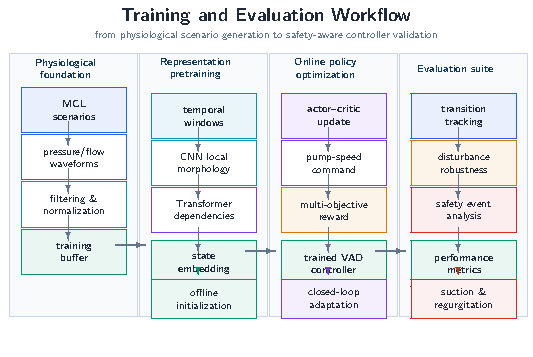
\includegraphics[width=\linewidth,trim=0 6mm 0 0,clip]{figures/training-evaluation-pipeline.pdf}
\vspace{-0.9em}
\caption{Training and evaluation pipeline of the proposed physiological VAD controller. The workflow links physiological scenario construction, signal preprocessing, CNN-Transformer representation pretraining, online actor-critic optimization, and downstream transition, robustness, safety, and ablation analyses.}
\label{fig:training_evaluation_pipeline}
\end{figure}
}{}

\subsection{Baseline and Evaluation Protocol}
The proposed method is evaluated against representative conventional and learning-based control strategies in order to examine both effectiveness and generality. Baseline methods are selected to reflect the main categories of VAD regulation approaches, including fixed-speed or rule-based controllers and existing deep reinforcement learning strategies. This comparison makes it possible to determine whether the proposed method provides meaningful improvements beyond both traditional control logic and previously reported learning-based designs.

The evaluation protocol includes three complementary parts: comparative experiments, robustness analysis, and ablation study. Comparative experiments are used to assess overall control quality under different physiological scenarios. Robustness analysis focuses on challenging conditions such as parameter perturbation, measurement noise, and abrupt physiological changes, which are important for determining whether the controller remains stable in safety-critical situations. The ablation study separately removes or replaces the CNN and Transformer components so that their individual contributions to physiological state representation and control performance can be examined.

The main evaluation criteria include physiological adaptability, hemodynamic regulation quality, control smoothness, and safety-related behavior. Particular attention is given to whether the controller can maintain appropriate support across changing operating conditions while avoiding unsafe regimes associated with suction, regurgitation, and hemolysis. Through this protocol, the experimental study is intended to provide a systematic assessment of both the effectiveness and the practical reliability of the proposed physiological control framework.

\section{Results and Discussion}
The experimental results are discussed from three aspects: comparative control performance, robustness and safety, and architectural ablation. This organization follows the evaluation protocol in Fig.~\ref{fig:training_evaluation_pipeline} and emphasizes whether the learned policy can maintain adaptive and stable VAD support across changing operating states.

\subsection{Comparative Control Performance}
In the comparative experiments, the proposed method is evaluated against representative baseline controllers during a rest-activity-recovery transition. This scenario tests whether the controller can match circulatory support to changing hemodynamic demand while preserving stable MAP regulation.

\IfFileExists{figures/comparative-control-performance-transitions.pdf}{
\begin{figure}[!htbp]
\centering
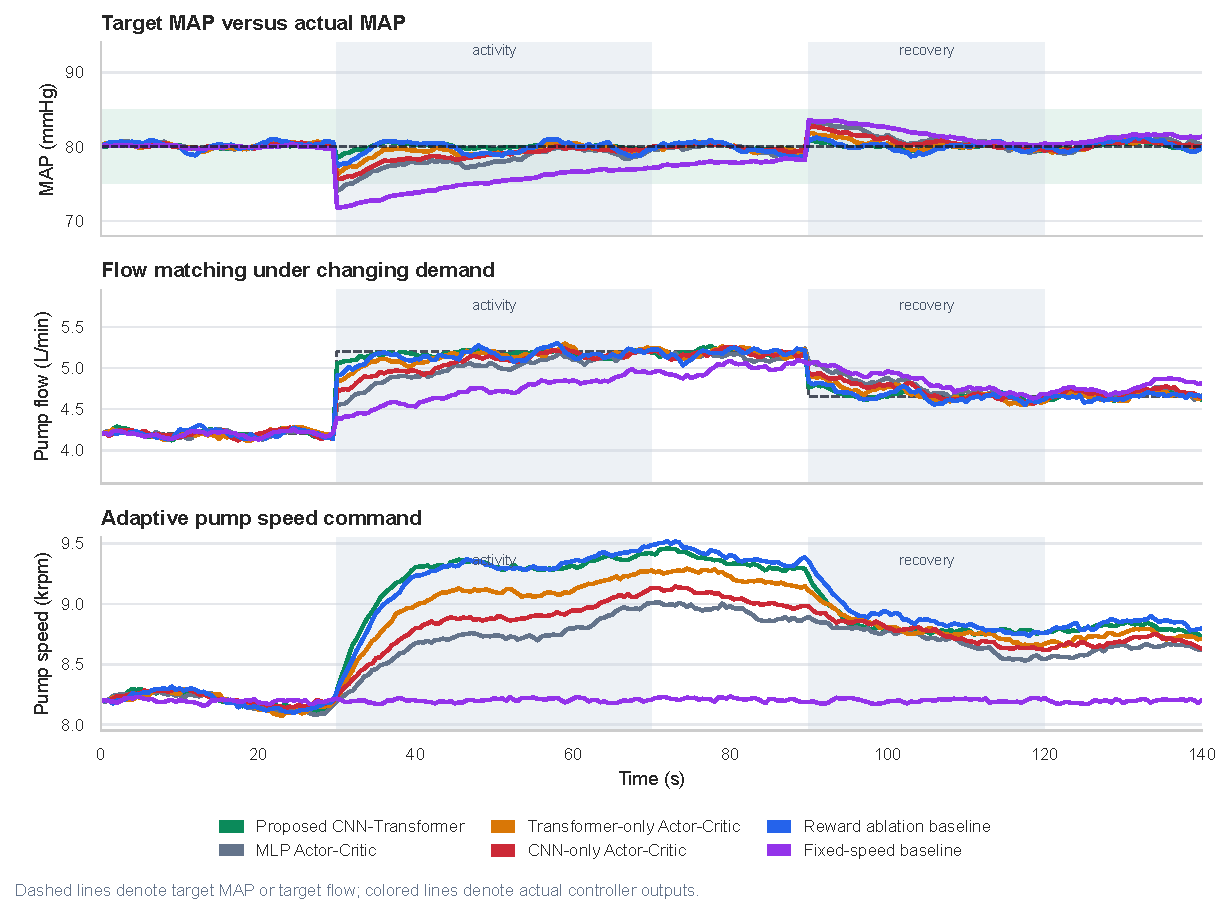
\includegraphics[width=\linewidth]{figures/comparative-control-performance-transitions.pdf}
\caption{Comparative MAP regulation during a rest-activity-recovery transition. The proposed CNN-Transformer controller is compared with existing DRL, rule-based, and fixed-speed baselines. The green band denotes the target MAP range, and the shaded windows mark the activity and recovery intervals.}
\label{fig:comparative_control_performance}
\end{figure}
}{}

As shown in Fig.~\ref{fig:comparative_control_performance}, the proposed CNN-Transformer controller maintains MAP within or close to the target band throughout the rest-activity-recovery transition, while the fixed-speed and rule-based baselines exhibit larger deviations immediately after the demand changes. These results indicate that the learned policy better matches circulatory support to time-varying physiological demand.

The MAP response in Fig.~\ref{fig:comparative_control_performance} further suggests that the proposed controller balances responsiveness and stability during both activity onset and recovery. Compared with weaker baselines, it reduces transient under-support after increased demand and avoids excessive overshoot when the operating condition returns toward rest.

\subsection{Robustness and Safety Analysis}
The robustness test focuses on composite disturbances that commonly challenge physiological VAD regulation, including sensor noise, preload drop, and afterload rise.

\IfFileExists{figures/robustness-safety-under-disturbances.pdf}{
\begin{figure}[!htbp]
\centering
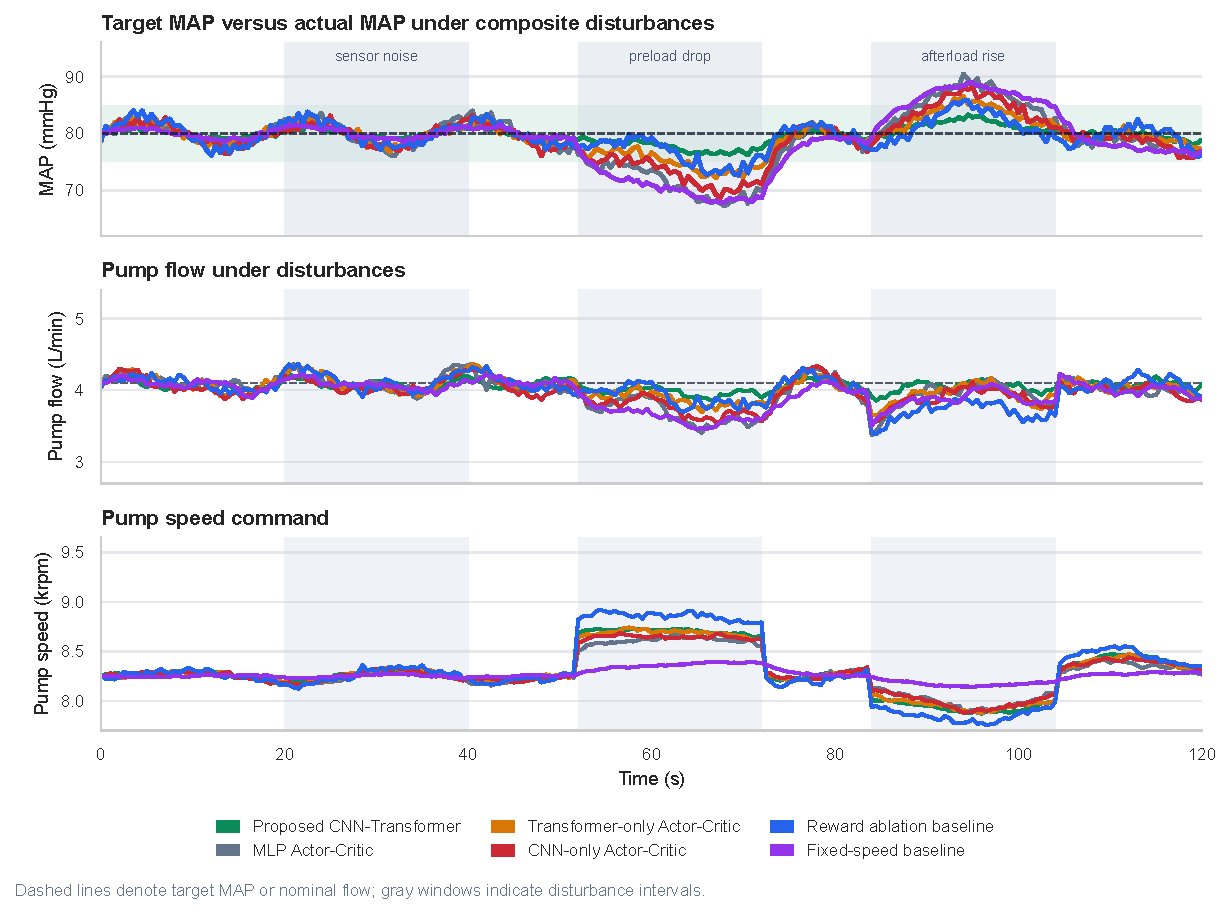
\includegraphics[width=\linewidth]{figures/robustness-safety-under-disturbances.pdf}
\caption{MAP response under composite disturbances. The proposed CNN-Transformer controller is compared with existing DRL and rule-based baselines during sensor noise, preload drop, and afterload rise intervals. The green band denotes the target MAP range, and the shaded windows mark the disturbance intervals.}
\label{fig:robustness_safety}
\end{figure}
}{}

Because VAD control is safety-critical, overall performance must be interpreted together with disturbance robustness and avoidance of unsafe operating regimes. The analysis therefore focuses on how each controller regulates MAP across the three disturbance windows.

Figure~\ref{fig:robustness_safety} shows that the proposed controller preserves a more stable hemodynamic response under composite disturbances than the baseline methods. The proposed method stays closer to the target band during noise injection, preload drop, and afterload rise, whereas the existing DRL and rule-based baselines display deeper excursions and slower recovery. This result indicates that the proposed policy is less sensitive to abrupt operating changes and can sustain acceptable perfusion during transient disturbances.

The response profile in Fig.~\ref{fig:robustness_safety} also suggests that the proposed controller avoids excessive overcorrection after the disturbances are removed. This behavior is important for VAD regulation because disturbance rejection should restore perfusion without introducing additional oscillation or unstable pump-support behavior.

\subsection{Ablation Study and Interpretation}
\IfFileExists{figures/ablation-performance-loss-heatmap.pdf}{
\begin{figure}[!htbp]
\centering
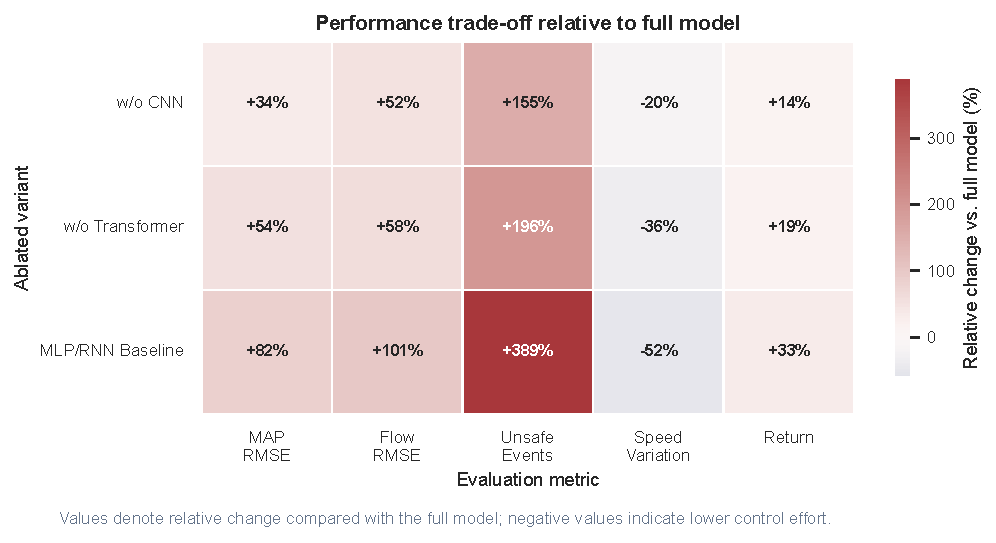
\includegraphics[width=\linewidth]{figures/ablation-performance-loss-heatmap.pdf}
\caption{Ablation study of CNN and Transformer modules using relative performance loss compared with the full model.}
\label{fig:ablation_study}
\end{figure}
}{}

The ablation analysis clarifies the contribution of the CNN and Transformer modules. By comparing the complete model with variants that weaken or remove local feature extraction and long-range temporal modeling, the experiments examine whether both components are necessary for physiological state representation.

As shown in Fig.~\ref{fig:ablation_study}, removing either module causes a consistent performance degradation compared with the full CNN-Transformer model, while the weaker MLP/RNN baseline performs worst overall. The relative-loss heatmap shows that the degradation is especially pronounced for unsafe-event control and speed variation, which suggests that both local waveform morphology and long-range temporal context are important for safety-aware adaptive control.

The ablation results further clarify the functional roles of the two components. The CNN mainly supports local morphological sensitivity, whereas the Transformer contributes to temporal adaptation and overall return. These results confirm that combining CNN-based local feature extraction with Transformer-based sequence modeling is central to the control quality of the proposed actor-critic controller.

\section{Conclusion}
This paper presented a deep reinforcement learning-based physiological control framework for ventricular assist devices. The method integrates an actor-critic learning scheme, a CNN-Transformer state representation model, and a multi-objective reward design to improve pump-speed regulation under nonlinear, time-varying, and safety-critical cardiovascular conditions.

The study established a systematic pipeline including physiologically relevant platform construction, staged model training, comparative transition evaluation, disturbance robustness analysis, and architectural ablation. The results show that the proposed controller improves perfusion matching, control smoothness, disturbance tolerance, and safety-related behavior compared with conventional and weaker learning-based baselines. Future work will focus on broader experimental validation, more complex pathological scenarios, and deployment on embedded and physical VAD platforms.

\begin{thebibliography}{00}
\bibitem{b1} N. Rajagopalan, B. Borlaug, A. Bailey, et al., ``Practical guidance for hemodynamic assessment by right heart catheterization in management of heart failure,'' \emph{J. Am. Coll. Cardiol. HF}, vol. 12, no. 7, pp. 1141--1156, 2024.
\bibitem{b2} D. Fernandez-Zapico, T. Peirelinck, G. Deconinck, et al., ``Physiological control for left ventricular assist devices based on deep reinforcement learning,'' \emph{Artificial Organs}, vol. 48, no. 12, pp. 1418--1429, 2024.
\bibitem{b3} C. Gross, L. Fresiello, and F. Moscato, ``Physiological control of left ventricular assist devices: A review of the past, present, and future,'' \emph{IEEE Rev. Biomed. Eng.}, vol. 15, pp. 187--202, 2022.
\bibitem{b4} T. Nishikawa, et al., ``Automated control of Impella maintains optimal left ventricular unloading during periods of unstable hemodynamics and prevents myocardial damage in acute myocardial infarction,'' \emph{Int. J. Cardiol.}, vol. 410, p. 132244, 2024.
\bibitem{b5} M. Azizkhani and Y. Chen, ``Supervised adaptive fuzzy control of LVAD with pulsatility ratio modulation,'' in \emph{Proc. IEEE 18th Int. Conf. Autom. Sci. Eng. (CASE)}, Mexico City, Mexico, 2022, pp. 2429--2434.
\bibitem{b6} H. Liu, A. Guan, F. Xing, et al., ``Cardiac index adaptive physiological control system for continuous-flow left ventricular assist device,'' \emph{Expert Syst. Appl.}, vol. 291, p. 128536, 2024.
\bibitem{b7} M. Bakouri, A. Alassaf, K. Alsharef, et al., ``An optimal H-infinity controller for left ventricular assist devices based on a Starling-like controller: A simulation study,'' \emph{Mathematics}, vol. 10, no. 5, p. 731, 2022.
\bibitem{b8} F. F. Haghighi, ``Deep learning methods for the estimation of preload and physiological control of heart assist devices,'' Ph.D. dissertation, Univ. New South Wales, Sydney, Australia, 2021.
\bibitem{b9} J. D. Willard, X. Jia, S. Xu, et al., ``Integrating physics-based modeling with machine learning: A survey,'' \emph{ACM Comput. Surv.}, vol. 55, no. 4, pp. 1--37, 2022.
\bibitem{b10} M. Bakouri, ``An advanced physiological control algorithm for left ventricular assist devices,'' \emph{Appl. Syst. Innov.}, vol. 6, no. 6, p. 97, 2023.
\bibitem{b11} S. Wang, Y. Teng, and P. Perdikaris, ``Understanding and mitigating gradient pathologies in physics-informed neural networks,'' \emph{SIAM J. Sci. Comput.}, vol. 43, no. 5, pp. A3055--A3081, 2021.
\bibitem{b12} M. Fetanat, M. Stevens, C. Hayward, et al., ``A sensorless control system for an implantable heart pump using a real-time deep convolutional neural network,'' \emph{IEEE Trans. Biomed. Eng.}, vol. 68, no. 10, pp. 3029--3038, 2021.
\bibitem{b13} D. Fernandez-Zapico, T. Peirelinck, G. Deconinck, et al., ``Physiological control for left ventricular assist devices based on deep reinforcement learning,'' \emph{Artif. Organs}, vol. 48, no. 12, pp. 1418--1429, 2024.
\bibitem{b14} Y. Y. Shi, Z. K. Xu, C. H. Chen, et al., ``Enhancing cardiac hemodynamic and pulsatility in heart failure via deep reinforcement learning: An in-silico and in-vitro validation study of percutaneous ventricular assist devices,'' \emph{Comput. Methods Programs Biomed.}, vol. 270, p. 108975, 2025.
\bibitem{b15} F. A. Gers, J. Schmidhuber, and F. Cummins, ``Learning to forget: Continual prediction with LSTM,'' \emph{Neural Comput.}, vol. 12, no. 10, pp. 2451--2471, 2000.
\bibitem{b16} T. Li, W. B. Cui, X. J. Liu, et al., ``A physiological control system for pulsatile ventricular assist device using an energy-efficient deep reinforcement learning method,'' \emph{IEEE Trans. Instrum. Meas.}, vol. 72, pp. 1--10, 2023.
\end{thebibliography}

\end{document}
